\newif\ifJPN
\JPNtrue
\JPNfalse

% Dropbox/pub/pgm/pgm-tehai.tex

\ifJPN
  \documentclass[a4paper,xelatex,ja=standard]{bxjsarticle}
\else
  \documentclass[a4paper,xelatex,english,ja=standard]{bxjsarticle}
\fi

%\setCJKmainfont[BoldFont=HaranoAjiMincho-Bold.otf]{HaranoAjiMincho-Regular.otf}
%\setCJKsansfont[BoldFont=HaranoAjiGothic-Bold.otf]{HaranoAjiGothic-Regular.otf}
\setCJKmonofont[BoldFont=HaranoAjiGothic-Bold.otf]{HaranoAjiGothic-Regular.otf}

\usepackage[style=authoryear, backend=biber]{biblatex} % BibLaTeX と Biber を使用
\addbibresource{koten.bib} % BibTeX ファイルを指定
\usepackage{tikz}
\usepackage{version}
\usepackage{amssymb}
\usepackage{amsmath}
\usepackage{booktabs} % このパッケージを追加
\usepackage{graphicx}
\usepackage{standalone}
\usepackage{url}
\usepackage{makeidx}
\usepackage{silence}
\WarningFilter{latexfont}{Font shape}
\WarningFilter{latexfont}{Some font shapes}
\WarningFilter{natbib}{There were undefined citations}
\WarningFilter{natbib}{Package natbib Warning}
\usepackage{metalogo} % \XeLaTeX ロゴのため
\usepackage{fancyvrb}
\usepackage{color}
\usepackage{amsmath}
\usepackage{listings} % シンプルで効果的なコードリスト表示
\lstset{
  language=Python,         % Pythonのシンタックスハイライト
  frame=t,            % 全体を枠線で囲む
  basicstyle=\ttfamily\footnotesize, % コードのフォントe定
  numbers=left,            % 行番号を左に表示
  numberstyle=\tiny,       % 行番号のフォントを小さくする
  stepnumber=1,            % 行番号を1行ごとに表示
  tabsize=4,               % タブのサイズを指定
  breaklines=true,         % 長い行を自動的に折り返す
  showstringspaces=false,  % 文字列の空白を表示しない
  keywordstyle=\color{blue}, % キーワードに色を付ける
  commentstyle=\color{black}, % コメントに色を付ける
  stringstyle=\color{red}, % 文字列に色を付ける
}
\usepackage{layout}
%\usepackage{natbib}
\usepackage{support-caption}
\usepackage[format=hang,labelsep=colon,margin=10pt,sc,normalsize]{caption}
%\captionsetup[table]{skip=0pt}
%\captionsetup[figure]{skip=10pt}
%\bibpunct[:\,]{(}{)}{,}{a}{}

\usepackage{hyperref}
\usepackage{url}
\usepackage{makeidx}

\makeindex

\ifJPN
%\captionsetup[table]{name=表}
%\captionsetup[figure]{name=図}
\renewcommand{\refname}{文献}
\renewcommand{\indexname}{索引}
\else
%\captionsetup[table]{name=Table~}
%\captionsetup[figure]{name=Figure~}
\renewcommand{\refname}{Reference}
\renewcommand{\indexname}{Index}
\fi

\if0
\newcounter{marginparcnt}[chapter]
\newcommand{\theMarginparcnt}{$\dagger$\arabic{marginparcnt}}
\newcommand{\Marginpar}[2][-7pt]{%
  \stepcounter{marginparcnt}%
  \textcolor{red}{\textsuperscript{\theMarginparcnt}}%
  \protect\marginpar{\vskip#1\footnotesize\color{blue}%
    \textsuperscript{\theMarginparcnt}
    {#2}\par}}
  \fi

\ifJPN
\title{連鎖維持を促進する「...て、はい、」の即時文法解析}
\author{
  山元 啓史\\東京科学大学
}
\else
\title{An Immediate Grammar Analysis of “...te, hai,” as a Chain-Maintenance Device in Japanese}
\author{
Hilofumi Yamamoto\\Institute of Science Tokyo
} 
\fi
\date{Last updated: \today}
\begin{document}
\maketitle

\ifJPN
\section{はじめに}
本稿は連鎖の維持を促進する表現「...て、はい、」の即時文法的特徴を解説したものである。
即時文法は、発話プロセスにおいて、不完全な文、言いさし表現を文法として捉える枠組みである。
感覚や雰囲気で理解されがちなこの表現を、体系的に理解するための手がかりを提供することを目的としている。
学習の初期に遭遇することが多いこの表現を適切に教材化すれば、学習者の混乱を軽減し、自然な日本語運用能力の向上に寄与できると考えられる\autocite{Yamamoto2025PGMv11}。
\else
\section{Introduction}
This paper explains the immediate grammatical features of the expression ``...te, hai," which promotes chain maintenance in Japanese conversation. Immediate grammar is a framework that treats incomplete sentences and trailing expressions as grammatical elements in the speech process. The purpose is to provide clues for systematically understanding this expression, which is often understood through intuition or atmosphere. 
Properly incorporating this expression into teaching materials, especially since learners often encounter it early in their studies, can reduce confusion and contribute to improving their natural Japanese language proficiency\autocite{Yamamoto2025PGMv11}.
\fi

\ifJPN
\else
\fi

\ifJPN
  \section{表現: 「...て、はい、」}
\else
  \section{Expression: ``...te, hai,"}
\fi

\ifJPN
例1: 連鎖維持表現「...て、はい、」の使用例
\begin{itemize}
  \item A「昨日、パーティ、どうだった」  
  \item B「まあ、食べて飲んで、はい、」  
  \item A「いつもと同じかぁ」
\end{itemize}
\else
Example 1: Usage of the Chain Maintenance Expression ``...te, hai,"

in Japanese Conversation
\begin{itemize}
  \item A: ``Kino, paatii, dou datta?"
  \item B: ``Maa, tabete nonde, hai,"
  \item A: ``Itsumo to onaji kaa"
\end{itemize}

in English:
\begin{itemize}
  \item A: ``How was the party yesterday?"  
  \item B: ``Well, I ate and drank, hai,"  
  \item A: ``Same as always, huh?"
\end{itemize}
\fi

\ifJPN
  \subsection{習得が難しいポイント}
\else
  \subsection{Difficult Points in Acquisition}
\fi

\ifJPN
  \subsubsection{「...て、」が未完了のまま 次に渡される}
問題点は、学習者は「て形=文をつなぐ文法」と学ぶが、この例では何と何をつないでいるかが明示されていない。
しかも 結論を明示しない。
例えば、上記の例では、

\begin{itemize}
  \item 食べて、飲んで、(それで?)
\end{itemize}

しかし、実際には「列挙した時点で、もう言うことは尽きている」という時間に即した判断が働いている\autocite{chafe1994}。
つまずきポイントとしては、「テ形の後には何か言わなければならない」と思い込むため、文法的な完結を探してしまうことである。
\else
  \subsubsection{``...te," is Left Incomplete and Passed to the Next Turn}
The issue is that learners are taught that the ``te-form" connects sentences, but in this example, it is not clear what is being connected. Moreover, the conclusion is not explicitly stated. For instance, in the above example:
\begin{itemize}
  \item Japanese: ``tabete, nonde, (sorede?)"
  \item English: ``Eating, drinking, (and then?)"
\end{itemize}
However, in reality, the judgment is made based on the timing that ``by the time the enumeration is done, there is nothing more to say."\autocite{chafe1994} A stumbling block is the assumption that ``something must be said after the te-form," leading learners to search for grammatical completeness.
\fi

\ifJPN
\subsubsection{「はい」が返事ではなく 会話の潤滑油になる}
問題点として、多くの教科書では「はい = yes / 返事」と教えられる。しかし、ここでは肯定でも応答でもない。
実際の機能としては、話し手がまだ話す権利を保持しつつ、「もう(内容的には)十分だよね?」という相手への確認を表す。これにより、相手への発話権の委譲がスムーズになる。
これは即時文法の典型で、意味ではなくタイミングの語である\autocite{duBois2007bstance}。
タイミングを示す語は、学習者にとって理解が難しいポイントであるだけでなく、教育者の意識や教材化の際にも見落とされがちな要素である。
\else
  \subsubsection{``hai" is not a Response but a Lubricant for Conversation}
The issue is that many textbooks teach ``hai = yes/response." However, in this context, it is neither an affirmation nor a response. Its actual function is to indicate that the speaker still retains the right to speak while confirming with the listener, ``Isn't that enough (in terms of content)?" This facilitates the smooth transfer of speaking rights to the listener. This is a typical feature of immediate grammar, where the word serves as a timing cue rather than conveying meaning (Du Bois, 2007).\autocite{duBois2007bstance} Timing cues are not only difficult for learners to understand but are also often overlooked by educators when creating teaching materials.
\fi

\ifJPN
  \subsubsection{情報伝達より「流れ」を優先する}
  この発話の目的は、内容を詳しく伝えるのでも、感想を述べるでもなく、会話を円滑に終わらせ、相手に続きを委ねることである\autocite{clark1996}。見方によれば、自分の発話権を手放すための表現とも言える。意図的に利用するならば、発話権を相手に移譲する信号を用いることによって、自分の不足している語彙量を相手に補完してもらうことができる。


学習者がこの言いさしを聞いている場合は「何を言っているのか」を理解しようとして失敗するが、「どこで息を渡しているか」、言い換えれば、「自分が話さなければならない番である」ことを感知し、コミュニケーションを継続し、成功させるのが課題となる。感知したら、どのような内容、あいづち、反応、表情でもよい。返答がなめらかに続けられれば、成功である。いわゆる「上手な聞き手」になる。
\else
  \subsubsection{Prioritizing ``Flow" over Information Transmission}
The purpose of this utterance is not to convey content in detail or to express impressions, but to smoothly conclude the conversation and entrust the continuation to the listener.\autocite{clark1996} From one perspective, it can be seen as an expression for relinquishing one's speaking rights. If used intentionally, it allows the speaker to signal the transfer of speaking rights to the listener, enabling them to supplement their own lack of vocabulary.

When learners hear this trailing expression, they may fail to understand ``what is being said," but the challenge is to sense ``where the breath is being passed," or in other words, to recognize ``it is their turn to speak," and to continue and succeed in communication. Once they sense this, any content, backchannel, reaction, or expression will suffice. Success is achieved when the response flows smoothly. This is what it means to be a ``good listener."
\fi

\ifJPN
  \subsubsection{調整文法では、同等の表現はない}
  この表現は伝統的な文法では表現されない\autocite{levinson1983}。
即時という時間的制約がないため、このようなやりとりは不要になる。
時間的余裕があり、情報伝達が優先される場合であれば、相手との距離を測りながら、いくぶん丁寧な表現が選択される。たとえば、

\begin{itemize}
  \item 即時:  ...て、はい、
  \item 調整:  ...して、そうですね、(何らかの評価語、例えば「おいしいですね」など)
\end{itemize}

このように、調整文法では明示的な評価語、丁寧な間投詞が必要になる。

学習者は「なぜ日本語話者は、そんなに短く済ませられるのか」と混乱するかもしれないが、今、まさにここで起こっているという即時的なインタラクションで十分な共有が成立しているからである。
\else
  \subsubsection{No Equivalent Expression in Adjustive Grammar}
This expression is not represented in traditional grammar.\autocite{levinson1983} Without the temporal constraint of immediacy, such interactions become unnecessary. When there is temporal leeway and information transmission is prioritized, somewhat polite expressions are chosen while gauging the distance with the interlocutor. For example:
\begin{itemize}
  \item Immediate:  ...te-form verb, hai(yes),
  \item Adjustive:  ...te-form verb, sou desu ne(well), (some evaluative phrase, e.g., ``oishii desu ne", meaning ``it's delicious, isn't it?")
\end{itemize}
Thus, in adjustive grammar, explicit evaluative phrases and polite interjections are necessary.
Learners may be confused about ``why Japanese speakers can get by with such brevity," but it is because sufficient shared understanding is established through the immediate interaction that is happening right here and now.
\fi

\ifJPN
  \subsection{この表現が「即時文法」だと一目でわかる理由}
\else
  \subsection{Why This Expression is Clearly ``Immediate Grammar"}
\fi


\ifJPN
  \begin{table}[htbp]\centering\small
    \caption{即時文法の特徴}\label{tab:immediate-grammar-features}
    \begin{tabular}[c]{ll}\noalign{\hrule height 0.8pt}
      要素 & 即時性       \\\hline
      テ形 & 結果を言わない       \\
      はい & 応答でも同意でもない \\
      文末 & 意図的に開いたまま   \\
      機能 & 情報 < タイミング    \\
    \end{tabular}
  \end{table}
\else
  \begin{table}[htbp]\centering\small
    \caption{Features of Immediate Grammar}\label{tab:immediate-grammar-features}
    \begin{tabular}[c]{ll}\noalign{\hrule height 0.8pt}
      Element & Immediacy       \\\hline
      Te-form & Does not state result       \\
      Hai & Neither response nor agreement \\
      Sentence End & Intentionally left open   \\
      Function & Information < Timing    \\
    \end{tabular}
  \end{table}
\fi


\ifJPN
表\ref{tab:immediate-grammar-features} は、不完全文がどのように相互行為を前進させるかを示す好例である。
文法構造の中に最終的な結論を示すノードが存在しない。
これは、発話が未完了であることを示している。
「食べて、飲んで、」は行為の列挙を示し、これ自体が完結した文ではない。
「はい、」は通常の応答や同意を示すものではなく、会話の流れを維持するための間投詞として機能している。
発話者は「はい、」を用いることで、自身の発話権を保持しつつ、相手に発話の機会を委譲する意図を示している。
これらは、従来の完全文を前提とした文法体系では説明できない特徴である。
\else
  Table \ref{tab:immediate-grammar-features} is a good example of how incomplete sentences advance interaction. There is no node in the grammatical structure that indicates a final conclusion. This indicates that the utterance is incomplete. ``I ate, drank," indicates an enumeration of actions and is not a complete sentence in itself. ``Hai," does not indicate a typical response or agreement but functions as an interjection to maintain the flow of conversation. By using ``hai," the speaker indicates their intention to retain their speaking rights while delegating the opportunity to speak to the listener. These are features that cannot be explained by traditional grammatical systems that assume complete sentences.
\fi



\ifJPN
\begin{figure}\centering\small
    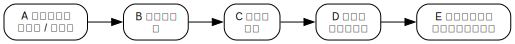
\includegraphics[width=0.95\textwidth]{./pgm-tehai-fig01-ja.pdf}
    \caption{連鎖維持装置「...て、はい、」の即時文法構造。ポイントは、どこにも「結論ノード」が存在しないことである。}\label{fig:immediate-grammar-structure}
\end{figure}
\else
  \begin{figure}\centering\small
    \includegraphics[width=0.95\textwidth]{./pgm-tehai-fig01-en.pdf}
    \caption{Immediate Grammar Structure of the Chain Maintenance Device ``...te, hai,". The key point is that there is no ``conclusion node" anywhere.}\label{fig:immediate-grammar-structure}
\end{figure}
\fi

\ifJPN
\begin{figure}[htbp]\centering\small
    \includegraphics[width=0.95\textwidth]{./pgm-tehai-fig02-ja.pdf}
    \caption{連鎖維持装置「...て、はい、」の即時インタラクションモデル。発話者が行為の列挙を提示し、未完了の状態を保持することで、受け手に次の発話ターンを誘発する\autocite{schegloff2007}。}\label{fig:immediate-interaction-model}
\end{figure}
\else
  \begin{figure}[htbp]\centering\small
    \includegraphics[width=0.95\textwidth]{./pgm-tehai-fig02-en.pdf}
    \caption{Immediate Interaction Model of the Chain Maintenance Device ``...te, hai,". The speaker presents an enumeration of actions and maintains an incomplete state, thereby inducing the listener to take the next speaking turn.\autocite{schegloff2007}}\label{fig:immediate-interaction-model}
\end{figure}
\fi

\ifJPN
\section{教材化するときのポイント}
教材化の際には、以下の点に注意する。「意味を説明しない」ことが重要である。意味ではなく、発話のタイミングに注目させる。意味を与えると正解を言わなければならないと考えてしまう。また、正解文を与えないことも重要である。学習者が自分で発話のタイミングを感じ取ることができるようにする。使われた位置だけを示し、学習者が自分で判断できるようにする。これを前後の発話とセットで提示する。評価は、発話がスムーズに続けられたかどうかで判断する。内容の正確さではない。
\else
\section{Points for Teaching Materials}
When creating teaching materials, it is important to focus on the timing of speech rather than its meaning. Providing meaning may lead learners to believe they must produce a correct answer. Additionally, it is crucial not to provide a ``correct" sentence. Instead, allow learners to sense the timing of their speech on their own. Indicate only where the expression is used, enabling learners to make their own judgments. Present this in conjunction with preceding and following utterances. Evaluation should be based on whether the speech flows smoothly, rather than the accuracy of the content.
\fi


\ifJPN
  \section{おわりに}
「...て、はい、」は
従来の記述文法的には壊れているが、
会話的には、発話の実態に即しており、パターンとして記述できる表現である。
情報伝達よりも会話の流れを重視しており、実際のコミュニケーションに即している。
なお、この表現は、AEAD number 627 (2025.12.28) に登録されている。
\else
  \section{Conclusion}
The expression ``...te, hai," may seem broken from the perspective of traditional descriptive grammar, but it accurately reflects the realities of spoken interaction and can be described as a pattern. It prioritizes the flow of conversation over mere information transmission, aligning well with actual communication practices. Notably, this expression is registered under AEAD number 627 (2025.12.28).
\fi


\printbibliography
\end{document}

Yamamoto2025PGM
